\documentclass{article}

\usepackage{amssymb, amsmath, amsthm, graphicx, tikz, tikz-3dplot}

\usepackage[pdftitle = {Assignment 5},
  pdfauthor = {Cameron Fredrickson},
  pdfsubject = {Typesetting},
  colorlinks = true,
  urlcolor = blue,
  linkcolor = blue,
  citecolor = blue]{hyperref}

% tikz default degrees, r option in "cos(\x r)" specifies radians

\title{Assignment 5}
\author{Cameron Fredrickson}
\date{}

\begin{document}

\maketitle

\begin{enumerate}
    \item The graph of the function \(x^2 - x\) on \(\left[0, 3\right]\), with the are underneath the curve on \(\left[1, 2\right]\) representing the area calculated by \(\int_1^2 \left(x^2 - x \right) \, dx\).
    \begin{center}
    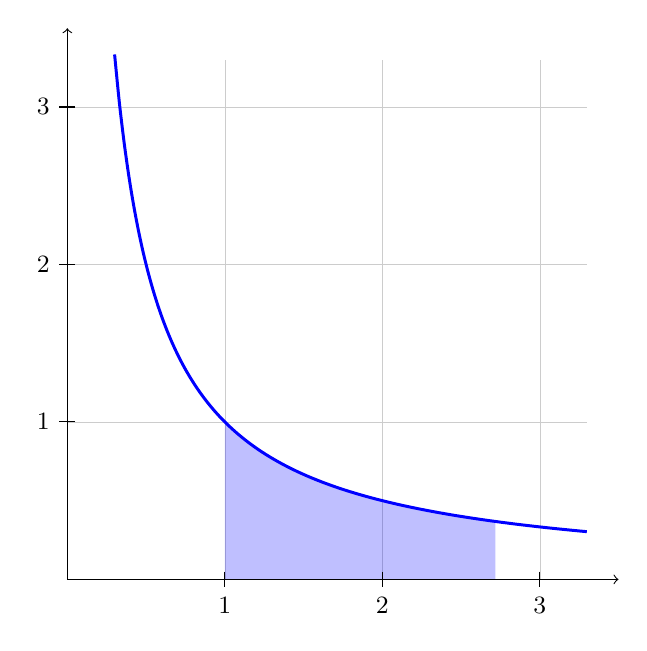
\begin{tikzpicture}[scale = 2]

    \draw [black!20, very thin] (0,0) grid (3.3,3.3);
    \fill [domain=1:e, smooth, blue, opacity = .25, samples = 100] (1,0) -- plot (\x, {pow(\x, -1)}) -- (e,0) -- cycle;
    \draw [domain=.3:3.3, smooth, line width = .25ex, blue, samples = 100] plot (\x, {pow(\x, -1)});
    \draw [->, thin] (0,0) -- (0,3.5);
    \draw [->, thin] (0,0) -- (3.5,0);
    \foreach \x in {1,2,3} {
      \draw (\x, .05) -- (\x, -.05) node [below] {\begin{small}$\x$\end{small}};
      \draw (.05, \x) -- (-.05, \x) node [left] {\begin{small}$\x$\end{small}};
    }
    \end{tikzpicture}
    \end{center}
\end{enumerate}

\end{document}